\documentclass[11pt]{article}

\usepackage{mhchem}
\usepackage{amsmath}
\usepackage{graphicx}

% Margins
\topmargin=-0.45in
\evensidemargin=0in
\oddsidemargin=0in
\textwidth=6.5in
\textheight=9.0in
\headsep=0.25in

\title{Thermochemistry Summary}
\author{Joseph Siu}
\date{\today}

\begin{document}
\maketitle	
\pagebreak

% Optional TOC
% \tableofcontents
% \pagebreak

%--Paper--

\section{Introduction to Thermochemistry}
\subsection{Changes in Matter and Energy}
\begin{itemize}
    \item Energy is the ability to do work
    \item Work is movement against a resistance
    \\
    \item Potential energy = stored energy as the result of position
    \item Kinetic energy = the energy of motion, $K_E=\frac{1}{2}mv^2$
    \item Unit = Joules (J), $1J=1\frac{kg\times m^2}{s^2}$
    \item Unit = Calories (cal) = the heat energy required to raise the temperature of 1 g of $\mathrm{H_2O}$ by $1^oC$, $1 \, \mathrm{ cal} = 4.184 \. J$
    \\
    \item Energy Changes
    \begin{itemize}
        \item Physical (hydrogen boils at -252$^oC$
        \item Chemical (hydrogen burns as fuel)
        \item Nuclear (hydrogen undergoes nuclear fusion in the Sun)
    \end{itemize}
    \\
    \item Thermal Energy = Total kinetic energy of all the particles in a material as a result of the motion of its molecules
    \item Temperature (T) = the average kinetic energy (energy of motion) of the particles in a material, measured in $^oC$ or K
    \item Heat (q) = Amount of energy transferred between two objects of different temperature, measured in Joules (J)
    \\
    \item Exothermic = releasing thermal energy, negative q value (q<0), increasing the temperature of the surrounding. 
    \item Endothermic = absorbing thermal energy, positive q value (q>0), decreasing the temperature of the surrounding.
    \item Specific Heat Capacity = The amount of energy required to raise the temperature of one gram of a substance by one $^oC$ or one K (different substances vary in their ability to absorb amounts of heat)
    \pagebreak
    \begin{equation}
        q=mc\Delta T
    \end{equation}
    The amount of heat transferred (q) depends on:
    \begin{enumerate}
        \item mass of sample (m) measured in grams
        \item temperature change ($\Delta T$) measured in $^oC$ or K
        \item specific heat capacity (c) measured in $\frac{J}{g\times ^oC}$ or $\frac{J}{g\times K}$
    \end{enumerate}
    \\
    \\
    \item Chemical Energy: Energy is required to break bonds (add energy) ; Energy is released when new bonds are formed (get energy)
        \begin{itemize}
            \item Liberate heat (exothermic) = energy to break $<$ energy to bond
            \item Absorb heat (endothermic) = energy to break $>$ energy to bond
        \end{itemize}
    \item Enthalpy of the reaction = the difference in energy (heat) between reactants and products
    \item Thermodynamics = The study of energy transformations that occur in a collection of matter
\end{itemize}

\subsection{Enthalpy changes ($\Delta H$)}
\begin{itemize}
    \item Thermodynamic systems
    \begin{itemize}
        \item Open
        \item Closed
        \item Isolated
    \end{itemize}
    \\

    \item The first law of Thermodynamics = the total energy of the universe is constant (energy can be neither destroyed nor created)
    \begin{itemize}
        \item It only transform from one form to another
        \begin{equation}
            \Delta E_{\text{universe}} = 0
        \end{equation}
    \end{itemize}
    \\
    
    \item Internal Energy
    \begin{itemize}
        \item Internal Energy = total energy of a system
        \item Cannot measure absolute internal energy
        \item Cannot measure change in internal energy
    \end{itemize}
    \\

    \item Energy cannot be created or destroyed
    \item Energy of (system + surroundings) is constant
    \item Any energy transferred from a system must be transferred to the surroundings (and vice verse)
    \item From the first law of thermodynamics:
    \begin{equation}
        \Delta E = q + w
    \end{equation}
    \begin{center}
        Change in energy = heat transferred + any work done
    \end{center}

    \pagebreak
    \item The amount of heat (energy) released or absorbed in a reaction carried out at constant pressure
    \item Standard enthalpy changes $\Delta H^\circ$ = Reactions done under standard conditions: 298K / 25$^\circ$C and pressure of 1 bar (100 kPa)
    \begin{itemize}
        \item $\Delta H^\circ_{r}$ = enthalpy of reaction
        \item $\Delta H^\circ_{f}$ = enthalpy of formation
        \item $\Delta H^\circ_{sol}$ = enthalpy of solution
        \item $\Delta H^\circ_{mel}$ = enthalpy of melting
        \item $\Delta H^\circ_{vap}$ = enthalpy of vaporization 
        \item $\Delta H^\circ_{x}$ = molar enthalpy = enthalpy change associated with a physical, chemical, or nuclear change involving one mole of a substance
    \end{itemize}
    \item Thermochemical equation = a balanced chemical equation that indicates the amount of heat that is absorbed or released by the reaction it represents
    \begin{align}
        \text{H}_{2(g)} + \frac{1}{2}\text{O}_{2(g)} &\xrightarrow{} \text{H}_2\text{O}_{(l)} \quad \Delta H_{rxn} = -285.8KJ \\
        \text{H}_{2(g)} + \frac{1}{2}\text{O}_{2(g)} &\xrightarrow{} \text{H}_2\text{O}_{(l)} + 285.8KJ
    \end{align}
    \item Enthalpy ($\Delta H$) is directly proportional to amount
    \item Change the sign of $\Delta H$ when the reaction is reversed
    \\

    \begin{equation}
        H=E+PV
    \end{equation}
    \begin{center}
        This is a state function (depends on the state of the system)
    \end{center}
    \item if the process occurs at constant pressure,
    \begin{equation}
        \Delta H = \Delta E + P\Delta V
    \end{equation}
    \item $\Delta H > 0$ if the system gains heat from the surroundings
    \item $\Delta H < 0$ if the surroundings gains heat from the system
    \\

    \begin{equation}
        \Delta H = n\Delta H_x
    \end{equation}
    \begin{center}
        n = # of moles\\
        $\Delta H_x$ = molar enthalpy ($\frac{KJ}{mol}$)
    \end{center}
    \\

    \item Activation Energy = The minimum quantity of energy needed by reacting species in order to undergo a reaction (usually the energy required to break the bonds)
\end{itemize}
\pagebreak
\subsection{Enthalpies of Formation}
\begin{itemize}
    \item Standard enthalpy of formation of the most stable form of an element is zero
    \item Using enthalpies of formation to calculate enthalpies of reactoin
    \begin{equation}
        \Delta H^\circ_{\text{rxn}} = \sum{n\cdot \Delta H_f^\circ} (\text{product}) - \sum{m\cdot \Delta H_f^\circ} (\text{reactants})
    \end{equation}
    \\

    \item Hess Law \\
    To find $A + B \xrightarrow{} C$,
    \begin{align*}
        A + B &\xrightarrow{} D \quad 4J\\
        D + E &\xrightarrow{} F \quad 7J\\
        F &\xrightarrow{} E + C \quad 14J
    \end{align*}
    Add them up,
    \begin{align*}
        A + B + D + E + F &\xrightarrow{} D + F + E + C \\
        A + B &\xrightarrow{} C \quad 25J
    \end{align*}
    \item The enthalpy change accompanying a chemical change is independent of the route by which the chemical change occurs.
    \item The overall enthalpy change will be exactly the same whether you do it in one step or two steps or however many steps
    \item Hess's law states that the standard reaction enthalpy is the sum of the standard enthalpies of the intermediate reactions into which the overall reaction can be divided (while temperature is constant)
    \item Hess's law allows us to calculate the enthalpy change for virtually any chemical reaction using a small set of standard data, starting from the elemental forms of each atom at 25$^\circ$C and 1 atm pressure.
    \\

    \item 1 nutritional Calorie, 1 Cal = 1000 cal = 1 kcal
    \item Fuel value = energy released when 1g of substance is burned
\end{itemize}


\pagebreak
\section{Calorimetry}
\begin{itemize}
    \item The science of measuring the change in heat of chemical reactions or physical changes
    \item A calorimeter: an insulated reaction vessel in which a reaction can occur and where the change in temperature of the system can be measured
\end{itemize}
Assumptions:
\begin{itemize}
    \item No heat is being transferred between the calorimeter and the outside environment (isolated system)
    \item Any heat absorbed or released by the calorimeter itself is negligible (unless information is given to you in the question)
    \item A dilute aqueous solution is assumed to have a density and specific heat capacity equal to that of water
    \item Cannot be used for reactions involving gases
    \item Cannot be used for high temperature reactions
\end{itemize}
Types of Calorimeters:
\begin{itemize}
    \item Coffee-Cup Calorimeter = Temperature difference of the water (aqueous solution) is measured, and using the equation $q=mc\Delta T$ we can find the heat released
    \item Bomb Calorimeter = $\Delta H_{\text{rxn}} = - q_\text{water}$, temperature difference of the water is measured
    \item Flame Calorimetry, measures enthalpy of combustion ($\Delta H_{comb} = - q_\text{total} = - q_\text{water} - q_\text{can}$)
\end{itemize}
Isolate the unknown,
\begin{align}
    m_w c_w \Delta T_w &= - m_x c_x \Delta T_x\\
    c_x &= \frac{m_w c_w \Delta T_w }{- m_x \Delta T_x}
\end{align}
\pagebreak

\section{Entropy and Gibbs Free Energy}
Entropy ($\Delta S$) = a measure of disorder or randomness

Increase in entropy = increase in disorder

The units for entropy are $\frac{J}{mol\cdot K}$

\newline\noindent Second Law of Thermodynamics = The entropy of the universe is constantly increasing

Molecules tend to become more and more disordered

$\Delta S = S_{\text{products}} - S_{\text{reactants}}$

\newline\noindent To solve for the entropy change of a reaction at standard conditions (SATP):
\begin{equation}
    \Delta S^\circ = \sum{n\cdot \Delta S^\circ_{\text{(products)}}} - \sum{n\cdot \Delta S^\circ_{\text{(reactants)}}}
\end{equation}

\noindent Gibbs Free Energy

Gibbs free energy is the energy that is available to do useful work. A reaction will spontaneously occur if free energy is negative (exergonic reaction), will not spontaneously occur if free energy is positive (endergonic reaction)

\begin{equation}
    \Delta G^\circ = \Delta H^\circ - T\Delta S^\circ
\end{equation}


\section{Chemical Kinetics (Rate of a Reaction)}
Methods to Measure Rate:
\begin{enumerate}
    \item pH Meter
    \item Spectroscopy (reactions in solution)
    \item Electrical conductance measurement (for ions)
    \item Pressure measurements (for reactions involving gases) 
\end{enumerate}

\begin{align}
    \text{rate} &\propto [\text{Br}_2]\\
    &= k[\text{Br}_2]\\
    k&=\frac{\text{rate}}{[\text{Br}_2]}
\end{align}

\noindent Reaction Rates and Stoichiometry

A mathematical expression that shows how the rate of the reaction depends on the concentrations of the specie sinvolved.

The rate expression may or may not be based on experimental data

\begin{align}
    aA + bB &\xrightarrow{} cC + dD \\
    \text{rate} = -\frac{1}{a}\frac{\Delta [A]}{\Delta t} = -\frac{1}{b}\frac{\Delta [B]}{\Delta t} &= \frac{1}{c}\frac{\Delta [C]}{\Delta t} = \frac{1}{d}\frac{\Delta [D]}{\Delta t} 
\end{align}

\noindent The Rate Law

The rate law expresses the relationship of the rate of a reaction to the rate constant and the [reactants] raised to some powers (must determined experimentally)

$aA+bB\xrightarrow{}cC+dD$

rate = $k[A]^x[B]^y$

$k = \frac{\text{rate}}{[A]^x[B]^y}$

where x and y are numbers must be determined experimentally 

gives the overall reaction order (defined as the sum of the powers to which all [reactants] are raised in the rate law)

$x^{th}$ order in A and $y^{th}$ order in B, and $(x+y)^{th}$ order overall

zero-order means that the rate is independent of the concentration of a particular reactant

\noindent Consider the decomposition of hydrogen peroxide at 20$^\circ$C;
\begin{align}
    2H_2O_{2(aq)} &\xrightarrow{} 2H_2O_{(l)} + O_{2(g)}\\
    PV&=nRT\\
    P&=\frac{n}{V}RT=[O_2]RT\\
    [O_2]&=\frac{1}{RT}P\\
    \text{rate}&=\frac{\Delta [O_2]}{\Delta t} = \frac{1}{RT}\frac{\Delta P}{\Delta t}\\
\end{align}

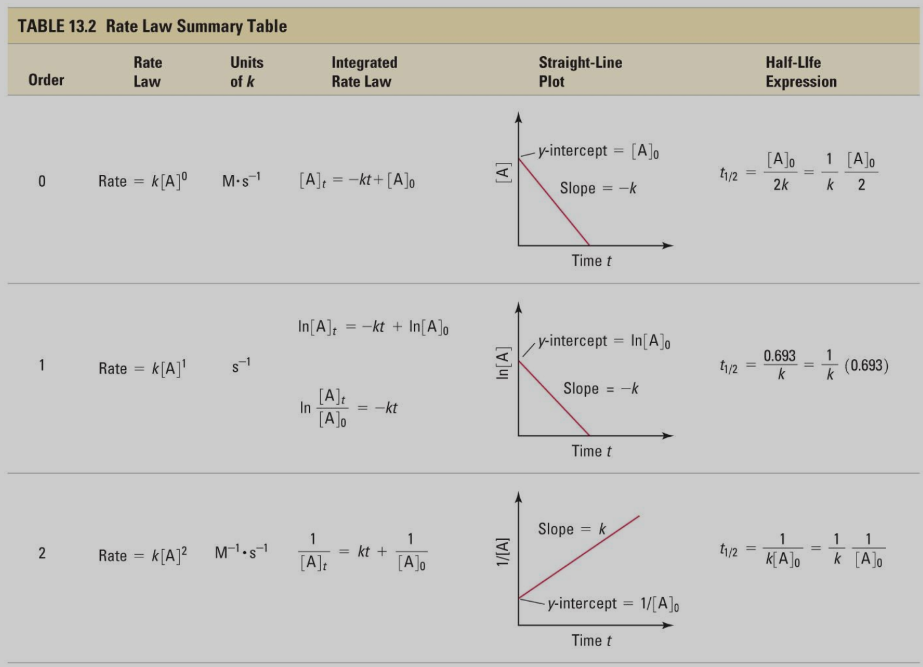
\includegraphics[scale=0.7]{ther2}

\pagebreak




\section{Formulas}
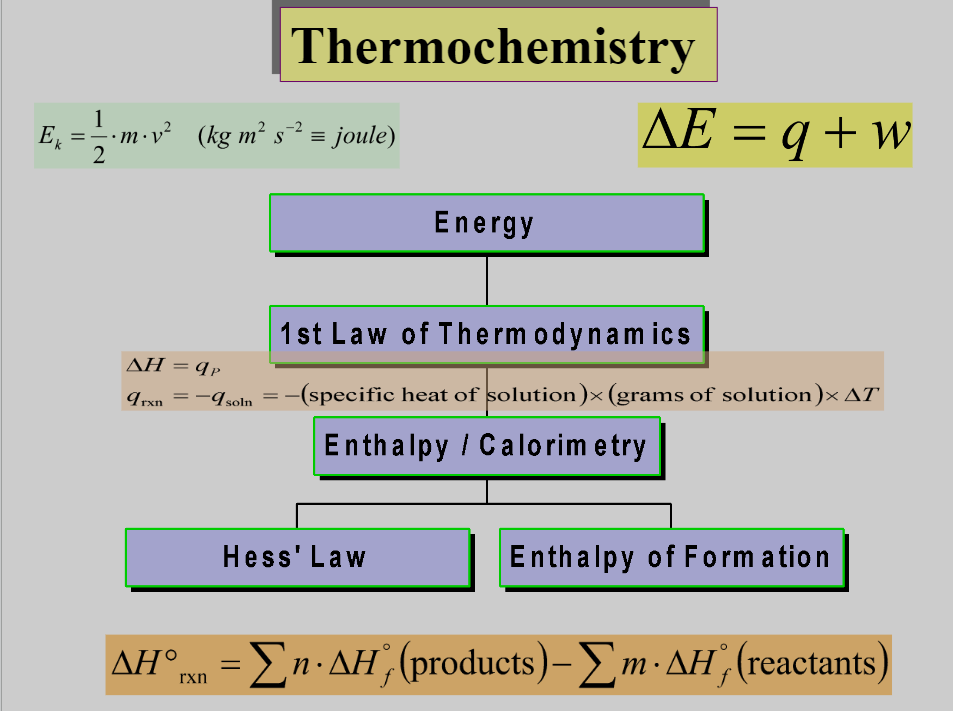
\includegraphics[scale=0.7]{ther1}

\end{document}